\begin{figure}[h!]
  \centering    
    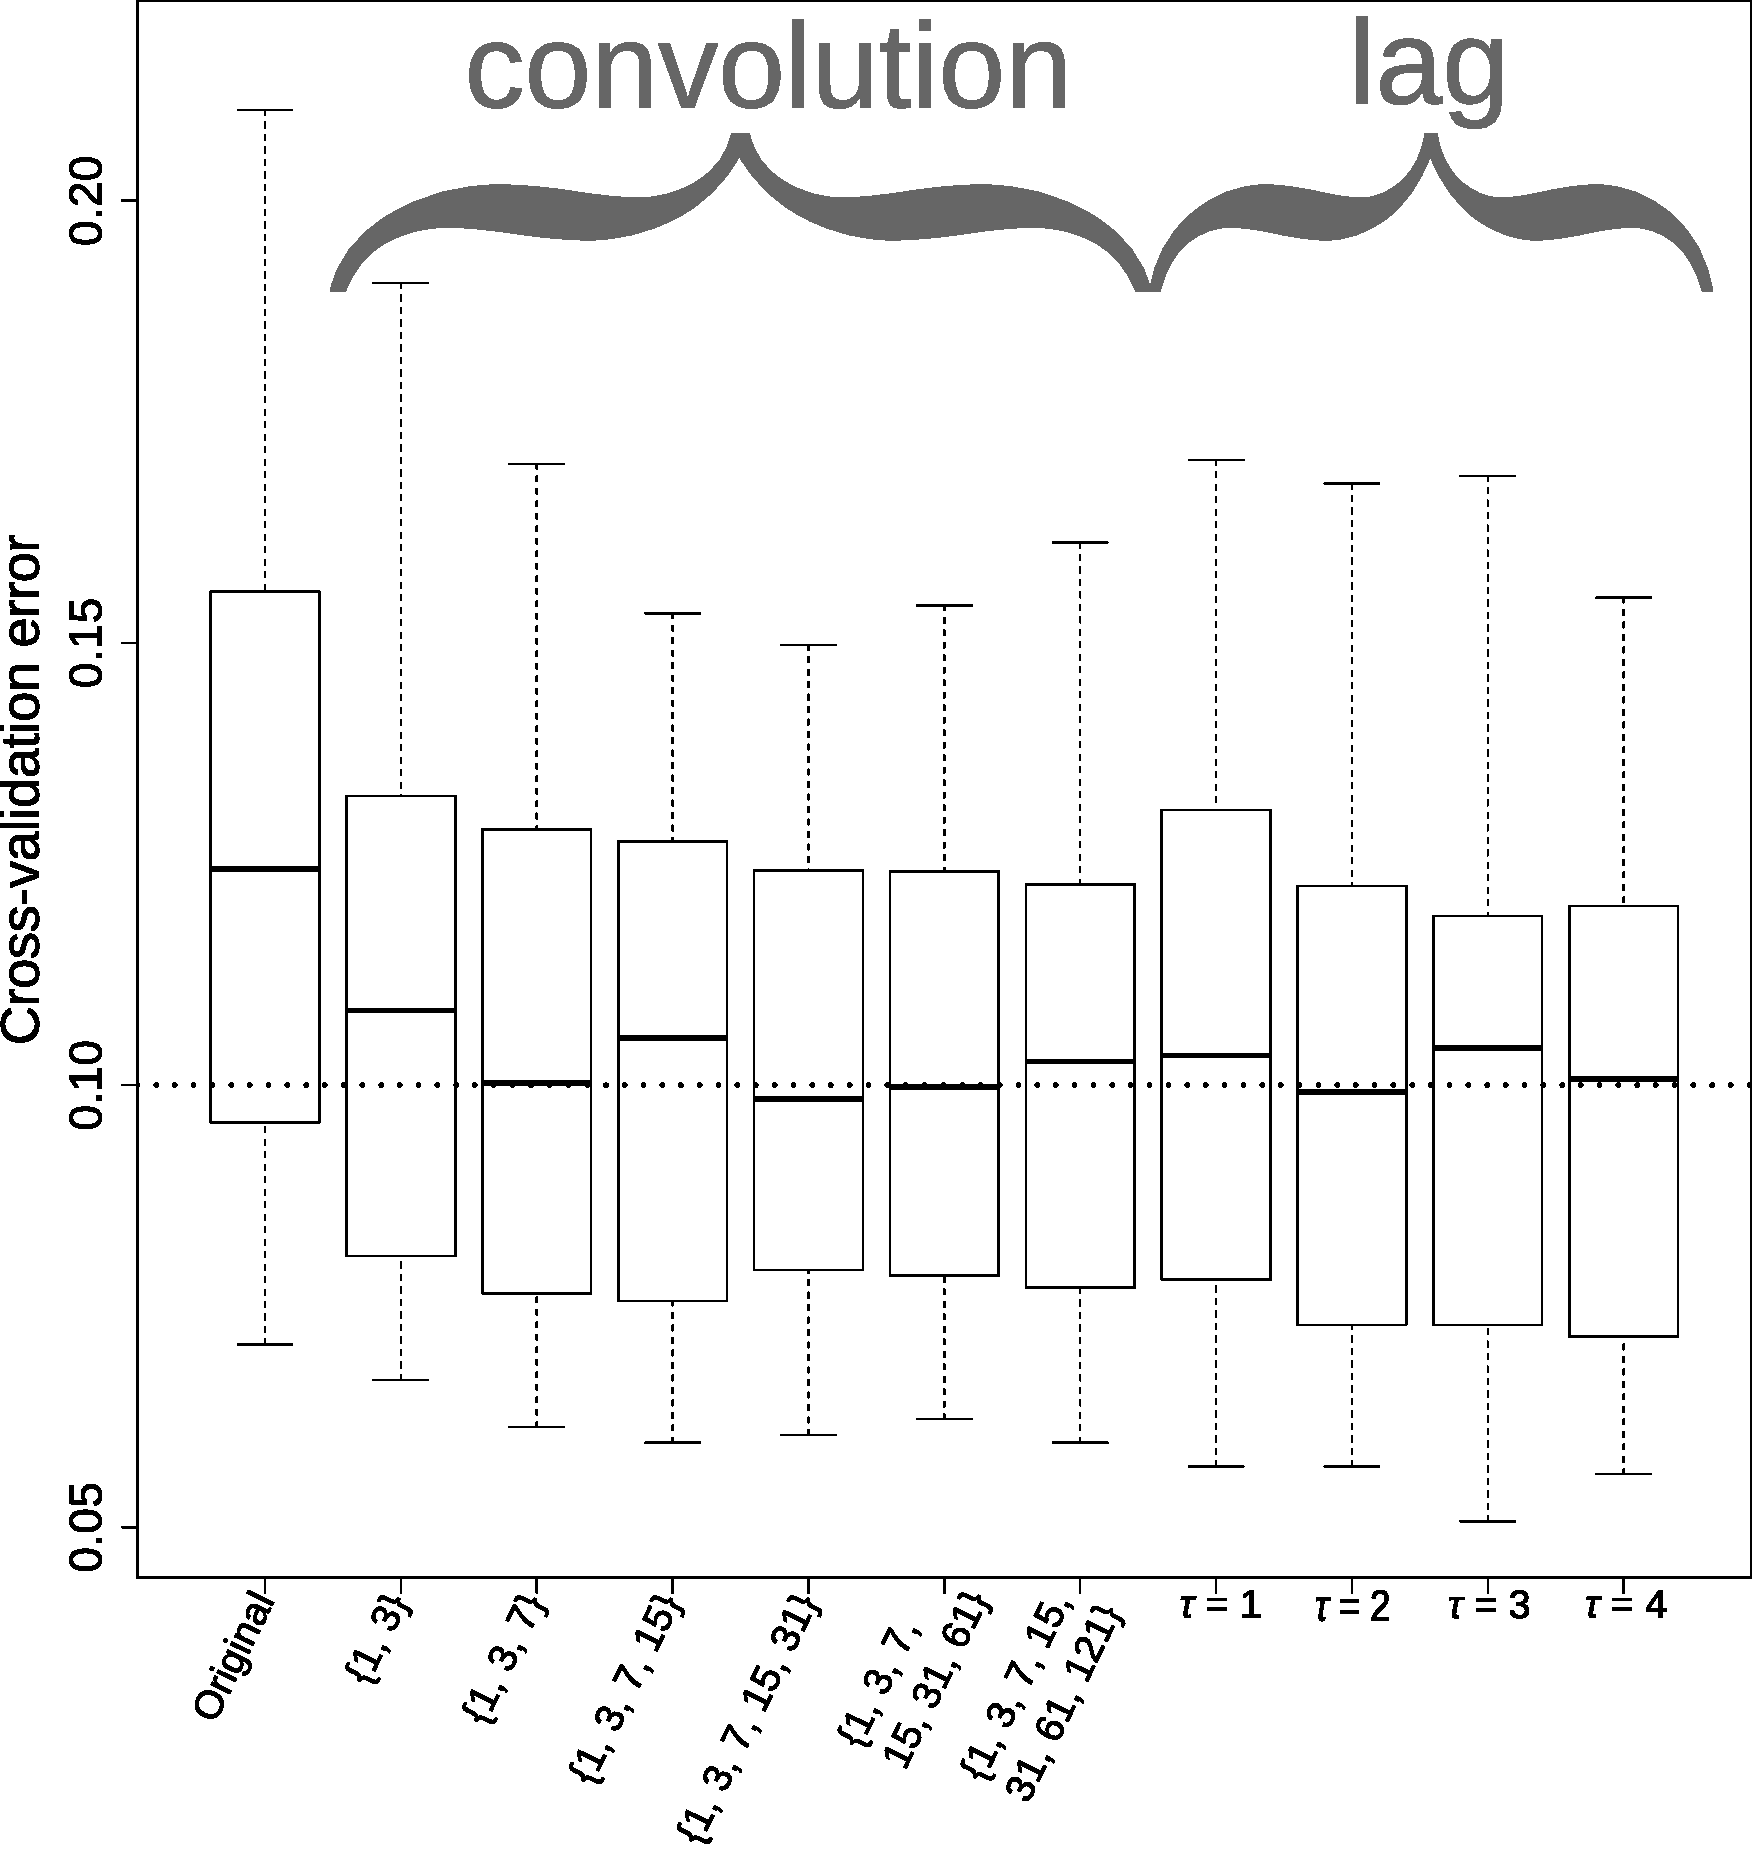
\includegraphics[width=0.95\textwidth]{figures/temporal_integration.pdf}
  \caption{\ctit{Integration of temporal information.}
  In order to improve prediction accuracy, information about the past and future features was added to the original features.
  Two different strategies were tested. Convolution involes inflating the vector of features by computing the mean features of neighbour points over, with different window size (eq.~\ref{eq:window}).
  The numbers in braces represent the window sizes. Alternatively, the features of the $\tau$ previous and future neighbours was added to the variables (eq.~\ref{eq:tau}).
  The dotted line reprents a cross-validation error of $10\%$
  \label{fig:temporal_integration}
  }
\end{figure}
